\documentclass[dvipsnames]{beamer}
\usepackage{../../shared/styles/custom}
\usepackage{../../shared/styles/conventions}

\title{Decision Trees \& Time Complexity}
\date{\today}
\author{Nipun Batra and teaching staff}
\institute{IIT Gandhinagar}

\setcounter{popquiz}{0}

\begin{document}
\maketitle

% Table of Contents
\begin{frame}{Table of Contents}
    \tableofcontents[hideallsubsections]
\end{frame}

\section{ID3 Algorithm for Decision Tree Building}

\begin{frame}{ID3 (Examples, Target Attribute, Attributes)}
\begin{itemize}[<*>]
    \item Create a root node for tree
    \item If all examples are +/-, return root with label = +/-
    \item  If attributes = empty, return root with most common value of
    Target Attribute in Examples
    \item Begin
    \begin{itemize}[<*>]
        \item A $\leftarrow$ attribute from Attributes which best classifies
        Examples
        \item 	Root $\leftarrow$ A
        \item  For each value (v) of A
        \begin{itemize}[<*>]
            \item Add new tree branch : A = v
            \item  Examples\textsubscript{v}: subset of examples that A = v
            \item If Examples\textsubscript{v}is empty: add leaf with label = most
            common value of Target Attribute
            \item Else: ID3 (Examples\textsubscript{v}, Target attribute, Attributes - {A})
        \end{itemize}
    \end{itemize}
\end{itemize}
\end{frame}

	\begin{frame}{Training Data}
\begin{tabular}{lllll||l} \toprule
	\textbf{Day} & \textbf{Outlook}  & \textbf{Temp} & \textbf{Humidity} & \textbf{Windy}  & \textbf{Play} \\ \midrule
	D1  & Sunny    & Hot  & High     & Weak   & No   \\
	D2  & Sunny    & Hot  & High     & Strong & No   \\
	D3  & Overcast & Hot  & High     & Weak   & Yes  \\
	D4  & Rain     & Mild & High     & Weak   & Yes  \\
	D5  & Rain     & Cool & Normal   & Weak   & Yes  \\
	D6  & Rain     & Cool & Normal   & Strong & No   \\
	D7  & Overcast & Cool & Normal   & Strong & Yes  \\
	D8  & Sunny    & Mild & High     & Weak   & No   \\
	D9  & Sunny    & Cool & Normal   & Weak   & Yes  \\
	D10 & Rain     & Mild & Normal   & Weak   & Yes  \\
	D11 & Sunny    & Mild & Normal   & Strong & Yes  \\
	D12 & Overcast & Mild & High     & Strong & Yes  \\
	D13 & Overcast & Hot  & Normal   & Weak   & Yes  \\
	D14 & Rain     & Mild & High     & Strong & No  \\ \bottomrule
\end{tabular}
\end{frame}


\begin{frame}{Entropy calculated}
We have 14 examples in $S$: 5 No, 9 Yes

$$\Entropy(S) = -p_{\text{No}} \log_2 p_{\text{No}} - p_{\text{Yes}} \log_2 p_{\text{Yes}}$$
$$
= -\frac{5}{14} \log_2\left(\frac{5}{14}\right) - \frac{9}{14} \log_2\left(\frac{9}{14}\right) = 0.940
$$
\end{frame}

\begin{frame}{Information Gain for Outlook}
\begin{tabular}{l|l} \toprule
\textbf{Outlook} & \textbf{Play} \\ \midrule
Sunny    & No   \\
Sunny    & No   \\
Overcast & Yes  \\
Rain     & Yes  \\
Rain     & Yes  \\
Rain     & No   \\
Overcast & Yes  \\
Sunny    & No   \\
Sunny    & Yes  \\
Rain     & Yes  \\
Sunny    & Yes  \\
Overcast & Yes  \\
Overcast & Yes  \\
Rain     & No  \\ \bottomrule
\end{tabular}
\end{frame}

\begin{frame}{Information Gain for Outlook}
\begin{columns}

\begin{column}<1->{.32\textwidth}
	\begin{table}
\begin{tabular}{l|l} \toprule
	\textbf{Outlook} & \textbf{Play} \\ \midrule
	Sunny    & No   \\
	Sunny    & No   \\
	Sunny    & No   \\
	Sunny    & Yes  \\
	Sunny    & Yes  \\

\bottomrule
\end{tabular}
We have 2 Yes, 3 No
$\Entropy = -\frac{3}{5} \log_2\left(\frac{3}{5}\right) - \frac{2}{5} \log_2\left(\frac{2}{5}\right) = 0.971$
\end{table}
\end{column}

\begin{column}<1->{.32\textwidth}
	\begin{table}
\begin{tabular}{l|l} \toprule
	\textbf{Outlook} & \textbf{Play} \\ \midrule

	Overcast & Yes  \\
	Overcast & Yes  \\
	Overcast & Yes  \\
	Overcast & Yes  \\ \bottomrule

\end{tabular}
We have 4 Yes, 0 No
$\Entropy = 0$ (pure subset)
	\end{table}
\end{column}

\begin{column}<1->{.32\textwidth}
	\begin{table}
\begin{tabular}{l|l} \toprule
	\textbf{Outlook} & \textbf{Play} \\ \midrule
	Rain     & Yes  \\
	Rain     & Yes  \\
	Rain     & No   \\
	Rain     & Yes  \\
	Rain     & No \\ \bottomrule
\end{tabular}
We have 3 Yes, 2 No
$\Entropy = -\frac{3}{5} \log_2\left(\frac{3}{5}\right) - \frac{2}{5} \log_2\left(\frac{2}{5}\right) = 0.971$
\end{table}
\end{column}
\end{columns}
\end{frame}

\begin{frame}{Information Gain}
\begin{align*}
\operatorname{Gain}(S, \text{Outlook}) 
&= \text{Entropy}(S) - \\
&\quad \sum_{v \in \{\text{Rain, Sunny, Overcast}\}} \frac{|S_{v}|}{|S|} \, \text{Entropy}(S_{v}) \\
\uncover<+-> {&= 0.940 - \frac{5}{14} \times 0.971 
     - \frac{4}{14} \times 0 
     - \frac{5}{14} \times 0.971} \\
&= 0.940 - 0.347 - 0 - 0.347 \\
&= 0.246
\end{align*}
\end{frame}

\begin{frame}{Information Gain}


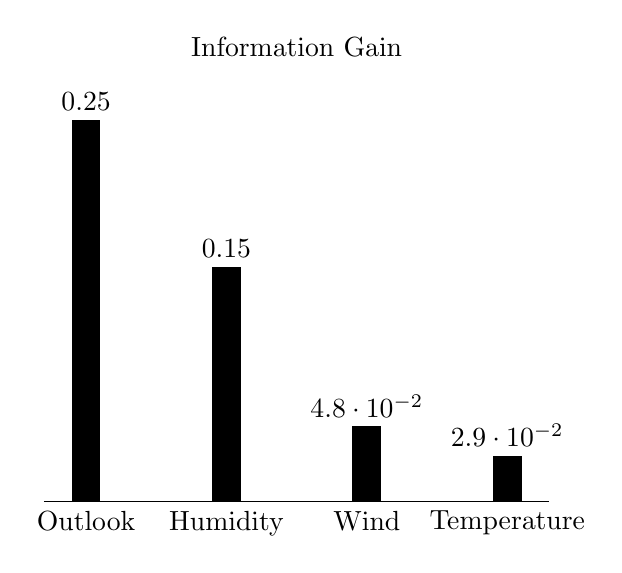
\begin{tikzpicture}
\begin{axis}[
symbolic x coords={Outlook,Humidity,Wind,Temperature},
xtick=data,xtick pos=left, width=8cm,
ytick pos=left,axis x line*=bottom,nodes near coords,hide y axis,title=Information Gain, ymin=0.0]
\addplot[ybar,fill=black] coordinates {
	(Outlook,0.246)
	(Humidity,0.151)
	(Wind,0.048)
	(Temperature,0.029)
};
\end{axis}
\end{tikzpicture}


\end{frame}

\begin{frame}{Learnt Decision Tree}
\begin{tikzpicture}[
node/.style={%
	draw,
	rectangle,
},
]

\node [node] (A) {Outlook};
\path (A) ++(-150:\nodeDist) node [node] (B) {?};
\path (A) ++(-90:\nodeDist/2) node [node, fill=green] (C) {Yes};
\path (A) ++(-30:\nodeDist) node [node] (D) {?};


\draw (A) -- (B) node [left,pos=0.25] {Sunny}(A);
\draw (A) -- (C) node [right,pos=0.8] {Overcast}(A);
\draw (A) -- (D) node [right,pos=0.5] {Rain}(A);

\end{tikzpicture}

\end{frame}

	\begin{frame}{Calling ID3 on Outlook=Sunny}
\begin{tabular}{llll||l} \toprule
	\textbf{Day} & \textbf{Temp} & \textbf{Humidity} & \textbf{Windy}  & \textbf{Play} \\ \midrule
	D1    & Hot  & High     & Weak   & No   \\
	D2     & Hot  & High     & Strong & No   \\
	D8     & Mild & High     & Weak   & No   \\
	D9    & Cool & Normal   & Weak   & Yes  \\
	D11    & Mild & Normal   & Strong & Yes  \\ \bottomrule
\end{tabular}

\begin{itemize}[<*>]
    \item Gain($S_{\text{Outlook=Sunny}}$, Temp) = Entropy(2 Yes, 3 No) - (2/5)*Entropy(0 Yes, 2 No) -(2/5)*Entropy(1 Yes, 1 No) - (1/5)*Entropy(1 Yes, 0 No) 
    \item Gain($S_{\text{Outlook=Sunny}}$, Humidity) = Entropy(2 Yes, 3 No) - (2/5)*Entropy(2 Yes, 0 No) -(3/5)*Entropy(0 Yes, 3 No) $\implies$ \textbf{maximum possible for the set}
    \item Gain($S_{\text{Outlook=Sunny}}$, Windy) = Entropy(2 Yes, 3 No) - (3/5)*Entropy(1 Yes, 2 No) -(2/5)*Entropy(1 Yes, 1 No) 
\end{itemize}
\end{frame}

\begin{frame}{Learnt Decision Tree}
\begin{tikzpicture}[
node/.style={%
	draw,
	rectangle,
},
]

\node [node] (A) {Outlook};
\path (A) ++(-150:\nodeDist) node [node] (B) {Humidity};
\path (A) ++(-90:\nodeDist/2) node [node, fill=green] (C) {Yes};
\path (A) ++(-30:\nodeDist) node [node] (D) {?};
\path (B) ++(-135:\nodeDist) node [node, fill=red] (E) {No};
\path (B) ++(-45:\nodeDist) node [node, fill=green] (F) {Yes};
;

\draw (A) -- (B) node [left,pos=0.25] {Sunny}(A);
\draw (A) -- (C) node [right,pos=0.8] {Overcast}(A);
\draw (A) -- (D) node [right,pos=0.5] {Rain}(A);
\draw (B) -- (E) node [left,pos=0.25] {High}(A);
\draw (B) -- (F) node [right,pos=0.25] {Normal}(C);

\end{tikzpicture}

\end{frame}


\begin{frame}{Calling ID3 on (Outlook=Rain)}
\begin{tabular}{llll||l} \toprule
	\textbf{Day}  & \textbf{Temp} & \textbf{Humidity} & \textbf{Windy}  & \textbf{Play} \\ \midrule
	D4    & Mild & High     & Weak   & Yes  \\
	D5     & Cool & Normal   & Weak   & Yes  \\
	D6      & Cool & Normal   & Strong & No   \\
	D10     & Mild & Normal   & Weak   & Yes  \\
	D14      & Mild & High     & Strong & No  \\ \bottomrule
\end{tabular}
\cleanitemize{
	\item The attribute Windy gives the highest information gain
}
\end{frame}

\begin{frame}{Learnt Decision Tree}
\begin{tikzpicture}[
node/.style={%
	draw,
	rectangle,
},
]

\node [node] (A) {Outlook};
\path (A) ++(-150:\nodeDist) node [node] (B) {Humidity};
\path (A) ++(-90:\nodeDist/2) node [node, fill=green] (C) {Yes};
\path (A) ++(-30:\nodeDist) node [node] (D) {Wind};
\path (B) ++(-135:\nodeDist) node [node, fill=red] (E) {No};
\path (B) ++(-45:\nodeDist) node [node, fill=green] (F) {Yes};
\path (D) ++(-45:\nodeDist) node [node, fill=red] (G) {No};
\path (D) ++(-135:\nodeDist) node [node, fill=green] (H) {Yes};

\draw (A) -- (B) node [left,pos=0.25] {Sunny}(A);
\draw (A) -- (C) node [right,pos=0.8] {Overcast}(A);
\draw (A) -- (D) node [right,pos=0.5] {Rain}(A);
\draw (B) -- (E) node [left,pos=0.25] {High}(A);
\draw (B) -- (F) node [right,pos=0.25] {Normal}(C);
\draw (D) -- (G) node [right,pos=0.25] {Strong}(A);
\draw (D) -- (H) node [left,pos=0.25] {Weak}(A);
\end{tikzpicture}

\end{frame}

% --- New Slides on DT Complexity ---
\section{DT Complexity Analysis}

% --- Slide 1
\begin{frame}{Goal \& Scope}
\cleanitemize{
    \item \textbf{Goal:} Build intuition for how Decision Tree runtime scales.
    \item \textbf{Scope:} Real inputs $\to$ 
    \begin{enumerate}
        \item Discrete output (classification: Gini/Entropy)
        \item Real output (regression: MSE)
    \end{enumerate}
    \item \textbf{Symbols:} 
    \cleanitemize{
        \item $N =$ number of samples
        \item $M =$ number of features
        \item $h =$ tree depth
        \item $S =$ samples at a given node
    }
}
\end{frame}

% --- Slide 2
\begin{frame}{Work at One Node}
\cleanitemize{
    \item We test axis-aligned splits: thresholds $x_j \leq t$ for each feature $j$.
    \item For a node with $S$ samples:
    \cleanitemize{
        \item Sort values of feature $j$ (or reuse sorted order).
        \item Consider up to $S-1$ midpoints as candidate thresholds.
        \item Sweep left $\to$ right, updating split quality.
    }
    \item Costs per feature at a node:
    \cleanitemize{
        \item With sorted order: $O(S)$ (one linear sweep).
        \item If sort here: $O(S \log S)$ sort + $O(S)$ scan $\Rightarrow O(S \log S)$.
    }
    \item Over all $M$ features: $O(MS)$ (presorted) vs. $O(M S \log S)$ (naïve).
}
\end{frame}
\begin{frame}{Training Data (Real Features)}
\begin{tabular}{llll||l} \toprule
	\textbf{Day} & \textbf{Temperature} & \textbf{Humidity} & \textbf{Wind Speed} & \textbf{Play} \\ \midrule
	D1  & 34.2 & 85 & 6.2  & No   \\
	D2  & 33.5 & 88 & 14.3 & No   \\
	D3  & 31.8 & 90 & 5.7  & Yes  \\
	D4  & 27.6 & 80 & 7.5  & Yes  \\
	D5  & 23.9 & 65 & 9.1  & Yes  \\
	D6  & 22.5 & 70 & 15.0 & No   \\
	D7  & 24.1 & 60 & 13.5 & Yes  \\
	D8  & 29.8 & 82 & 6.8  & No   \\
	D9  & 25.3 & 72 & 7.0  & Yes  \\
	D10 & 26.7 & 68 & 8.2  & Yes  \\
	D11 & 28.9 & 75 & 12.0 & Yes  \\
	D12 & 30.5 & 89 & 11.5 & Yes  \\
	D13 & 32.0 & 70 & 5.9  & Yes  \\
	D14 & 27.2 & 85 & 13.2 & No   \\ \bottomrule
\end{tabular}
\end{frame}

% --- Slide 4
\begin{frame}{Training Complexity: Efficient Implementation}
\cleanitemize{
    \item Presort once per feature at the root: $O(M N \log N)$.
    \item Children inherit sorted order by partitioning.
    \item At any level, total samples processed $= N$.
    \item Over depth $h$ (balanced $\approx \log_2 N$): total mass = $N \cdot h$.
    \item Per level: $O(MN)$, across $h$ levels: $O(MNh)$.
    \item Add presort $O(MN \log N)$ $\Rightarrow$ overall $O(MN \log N)$.
}
\onslide<7->\textbf{Result (both tasks):} Train $= O(MN \log N)$.
\end{frame}

% --- Slide 5
\begin{frame}{Training Complexity: Naïve (Re-sorting)}
\cleanitemize{
    \item If re-sort at each node:
    \cleanitemize{
        \item Node cost: $O(M S \log S)$.
        \item Level $\ell$: $2^\ell$ nodes of size $\approx N/2^\ell$.
        \item Level cost: $M N (\log N - \ell)$.
    }
    \item Sum over $\ell = 0$ to $h-1$ ($h \approx \log N$):
    \begin{align*}
        \sum M N (\log N - \ell) &= M N \cdot \frac{(\log N)(\log N+1)}{2}.
    \end{align*}
    \item Complexity: $O(M N (\log N)^2)$.
}
\onslide<7->\textbf{Result:} Train $= O(MN(\log N)^2)$ if you re-sort.
\end{frame}

% --- Slide 6
\begin{frame}{Prediction Complexity}
\cleanitemize{
    \item Each test point follows one path root $\to$ leaf.
    \item Per sample: $O(h)$ comparisons.
    \item For $N_{\text{test}}$ points: $O(N_{\text{test}} h)$.
    \item Balanced: $h \approx \log N \Rightarrow O(N_{\text{test}} \log N)$.
    \item Worst case (unbalanced): $h = \Theta(N) \Rightarrow O(N_{\text{test}} N)$.
}
\end{frame}

% --- Slide 7
\begin{frame}{Classification vs Regression}
\cleanitemize{
    \item Same asymptotics: $O(M N \log N)$ train, $O(N_{\text{test}} h)$ predict.
    \item Difference is only in constants:
    \cleanitemize{
        \item Entropy slower than Gini (logs).
        \item MSE similar to Gini.
    }
    \item Binary features: no sorting needed, but per-level scan still linear. What about fixed discrete features?
}
\end{frame}

% --- Slide 3
\begin{frame}{APPENDIX: Why the Sweep is Linear}
\textbf{Classification (real $\to$ discrete):}
\cleanitemize{
    \item Maintain class counts $(c_L, c_R)$.
    \item Update counts in $O(1)$ as samples shift.
    \item Compute Gini $= 1 - \sum p_k^2$ or Entropy $= -\sum p_k \log p_k$ in $O(1)$.
    \item $\Rightarrow$ Whole sweep per feature: $O(S)$.
}

\onslide<5->{\textbf{Regression (real $\to$ real):}
\cleanitemize{
    \onslide<5->{\item Maintain $(\sum y, \sum y^2, n)$ for left; right = totals $-$ left.}
    \onslide<6->{\item SSE $= \sum y^2 - (\sum y)^2/n$, updated in $O(1)$.}
    \onslide<7->{\item $\Rightarrow$ Whole sweep per feature: $O(S)$.}
}
}

\onslide<8->\textbf{Takeaway:} Both Gini/Entropy and MSE need linear sweeps.
\end{frame}

\end{document}